\documentclass[12pt,a4paper]{article}
\usepackage[utf8]{inputenc}
\usepackage[portuguese]{babel}
\usepackage[margin=2.5cm]{geometry}
\usepackage{url}
\usepackage{amsmath}
\usepackage{amsfonts}
\usepackage{amssymb}
\usepackage{graphicx}

\title{MAC0344 Arquitetura de Computadores\\Lista de Exercícios No. 1}
\author{Aluno: Leonardo Heidi Almeida Murakami \\ NUSP: 11260186}
\date{\today}

\begin{document}

\maketitle

\section*{Questão 1}

\textbf{Na lista top500 de junho deste ano (consultar o site top500.org), quais os computadores instalados no Brasil?}

Consultando a lista TOP500 de junho de 2025, foram encontrados \textbf{nove} computadores brasileiros:

\subsection*{1. Pégaso}
\begin{itemize}
    \item \textbf{Posição no ranking:} 86º lugar
    \item \textbf{Instituição:} Petróleo Brasileiro S.A. (Petrobras)
    \item \textbf{Localização:} Vargem Grande, Rio de Janeiro, Brasil
    \item \textbf{Número de cores:} 233.856 cores
    \item \textbf{Velocidade Linpack (Rmax):} 19,07 PFLOPS
    \item \textbf{Velocidade de pico (Rpeak):} 42,00 PFLOPS
    \item \textbf{Fabricante:} EVIDEN
    \item \textbf{Sistema:} Supermicro A+ Server 4124GO-NART+, AMD EPYC 7513 32C 2.6GHz, NVIDIA A100, Infiniband HDR
    \item \textbf{Consumo de energia:} 1.033 kW
\end{itemize}

\newpage
\subsection*{2. Santos Dumont}
\begin{itemize}
    \item \textbf{Posição no ranking:} 107º lugar
    \item \textbf{Instituição:} Laboratório Nacional de Computação Científica (LNCC)
    \item \textbf{Localização:} Petrópolis, Rio de Janeiro, Brasil
    \item \textbf{Número de cores:} 68.064 cores
    \item \textbf{Velocidade Linpack (Rmax):} 14,29 PFLOPS
    \item \textbf{Velocidade de pico (Rpeak):} 20,26 PFLOPS
    \item \textbf{Fabricante:} EVIDEN
    \item \textbf{Sistema:} BullSequana XH3000, Grace Hopper Superchip 72C 3GHz, NVIDIA GH200 Superchip, Quad-Rail NVIDIA InfiniBand NDR200, Red Hat Enterprise Linux
    \item \textbf{Consumo de energia:} 312 kW
\end{itemize}

\subsection*{3. Dragão}
\begin{itemize}
    \item \textbf{Posição no ranking:} 160º lugar
    \item \textbf{Instituição:} Petróleo Brasileiro S.A. (Petrobras)
    \item \textbf{Localização:} Rio de Janeiro, Brasil
    \item \textbf{Número de cores:} 188.224 cores
    \item \textbf{Velocidade Linpack (Rmax):} 8,98 PFLOPS
    \item \textbf{Velocidade de pico (Rpeak):} 14,01 PFLOPS
    \item \textbf{Fabricante:} EVIDEN
    \item \textbf{Sistema:} Supermicro SYS-4029GP-TVRT, Xeon Gold 6230R 26C 2.1GHz, NVIDIA Tesla V100, Infiniband EDR
    \item \textbf{Consumo de energia:} 943 kW
\end{itemize}

\newpage
\subsection*{4. Gaia}
\begin{itemize}
    \item \textbf{Posição no ranking:} 193º lugar
    \item \textbf{Instituição:} Petróleo Brasileiro S.A. (Petrobras)
    \item \textbf{Localização:} Rio de Janeiro, Brasil
    \item \textbf{Número de cores:} 84.480 cores
    \item \textbf{Velocidade Linpack (Rmax):} 6,97 PFLOPS
    \item \textbf{Velocidade de pico (Rpeak):} 13,73 PFLOPS
    \item \textbf{Fabricante:} DELL
    \item \textbf{Sistema:} PowerEdge XE8545, AMD EPYC 74F3 24C 3.2GHz, NVIDIA A100, Infiniband
    \item \textbf{Consumo de energia:} 574 kW
\end{itemize}

\subsection*{5. Atlas}
\begin{itemize}
    \item \textbf{Posição no ranking:} 265º lugar
    \item \textbf{Instituição:} Petróleo Brasileiro S.A. (Petrobras)
    \item \textbf{Localização:} Rio de Janeiro, Brasil
    \item \textbf{Número de cores:} 91.936 cores
    \item \textbf{Velocidade Linpack (Rmax):} 4,38 PFLOPS
    \item \textbf{Velocidade de pico (Rpeak):} 8,85 PFLOPS
    \item \textbf{Fabricante:} EVIDEN
    \item \textbf{Sistema:} Bull 4029GP-TVRT, Xeon Gold 6240 18C 2.6GHz, NVIDIA Tesla V100, Infiniband EDR
    \item \textbf{Consumo de energia:} 547 kW
\end{itemize}

\newpage
\subsection*{6. Gemini}
\begin{itemize}
    \item \textbf{Posição no ranking:} 303º lugar
    \item \textbf{Instituição:} Petróleo Brasileiro S.A. (Petrobras)
    \item \textbf{Localização:} Rio de Janeiro, Brasil
    \item \textbf{Número de cores:} 42.240 cores
    \item \textbf{Velocidade Linpack (Rmax):} 3,86 PFLOPS
    \item \textbf{Velocidade de pico (Rpeak):} 6,86 PFLOPS
    \item \textbf{Fabricante:} DELL
    \item \textbf{Sistema:} PowerEdge XE8545, AMD EPYC 74F3 24C 3.2GHz, NVIDIA A100, Infiniband
    \item \textbf{Consumo de energia:} 287 kW
\end{itemize}

\subsection*{7. IARA}
\begin{itemize}
    \item \textbf{Posição no ranking:} 312º lugar
    \item \textbf{Instituição:} SiDi (Sistemas de Informação Distribuída)
    \item \textbf{Localização:} Brasil
    \item \textbf{Número de cores:} 24.800 cores
    \item \textbf{Velocidade Linpack (Rmax):} 3,66 PFLOPS
    \item \textbf{Velocidade de pico (Rpeak):} 4,13 PFLOPS
    \item \textbf{Fabricante:} Nvidia
    \item \textbf{Sistema:} NVIDIA DGX A100, AMD EPYC 7742 64C 2.25GHz, NVIDIA A100 SXM4 40 GB, Infiniband
    \item \textbf{Consumo de energia:} Não informado
\end{itemize}

\newpage
\subsection*{8. NOBZ1}
\begin{itemize}
    \item \textbf{Posição no ranking:} 325º lugar
    \item \textbf{Instituição:} Software Company MBZ
    \item \textbf{Localização:} Brasil
    \item \textbf{Número de cores:} 80.640 cores
    \item \textbf{Velocidade Linpack (Rmax):} 3,55 PFLOPS
    \item \textbf{Velocidade de pico (Rpeak):} 6,97 PFLOPS
    \item \textbf{Fabricante:} Lenovo
    \item \textbf{Sistema:} ThinkSystem C2397, Xeon Platinum 8280 28C 2.7GHz, Broadcom
    \item \textbf{Consumo de energia:} Não informado
\end{itemize}

\subsection*{9. Fênix}
\begin{itemize}
    \item \textbf{Posição no ranking:} 355º lugar
    \item \textbf{Instituição:} Petróleo Brasileiro S.A. (Petrobras)
    \item \textbf{Localização:} Rio de Janeiro, Brasil
    \item \textbf{Número de cores:} 60.480 cores
    \item \textbf{Velocidade Linpack (Rmax):} 3,16 PFLOPS
    \item \textbf{Velocidade de pico (Rpeak):} 5,37 PFLOPS
    \item \textbf{Fabricante:} EVIDEN
    \item \textbf{Sistema:} Bull 4029GP-TVRT, Xeon Gold 5122 4C 3.6GHz, NVIDIA Tesla V100, Infiniband EDR
    \item \textbf{Consumo de energia:} 390 kW
\end{itemize}

\newpage
\section*{Questão 2}

\textbf{Procure um gráfico na internet comparando o avanço do processador versus o avanço da memória, em termos de desempenho (performance), e responda qual dos dois avança mais em relação ao outro.}

\subsection*{Gráfico:}

\begin{figure}[h]
    \centering
    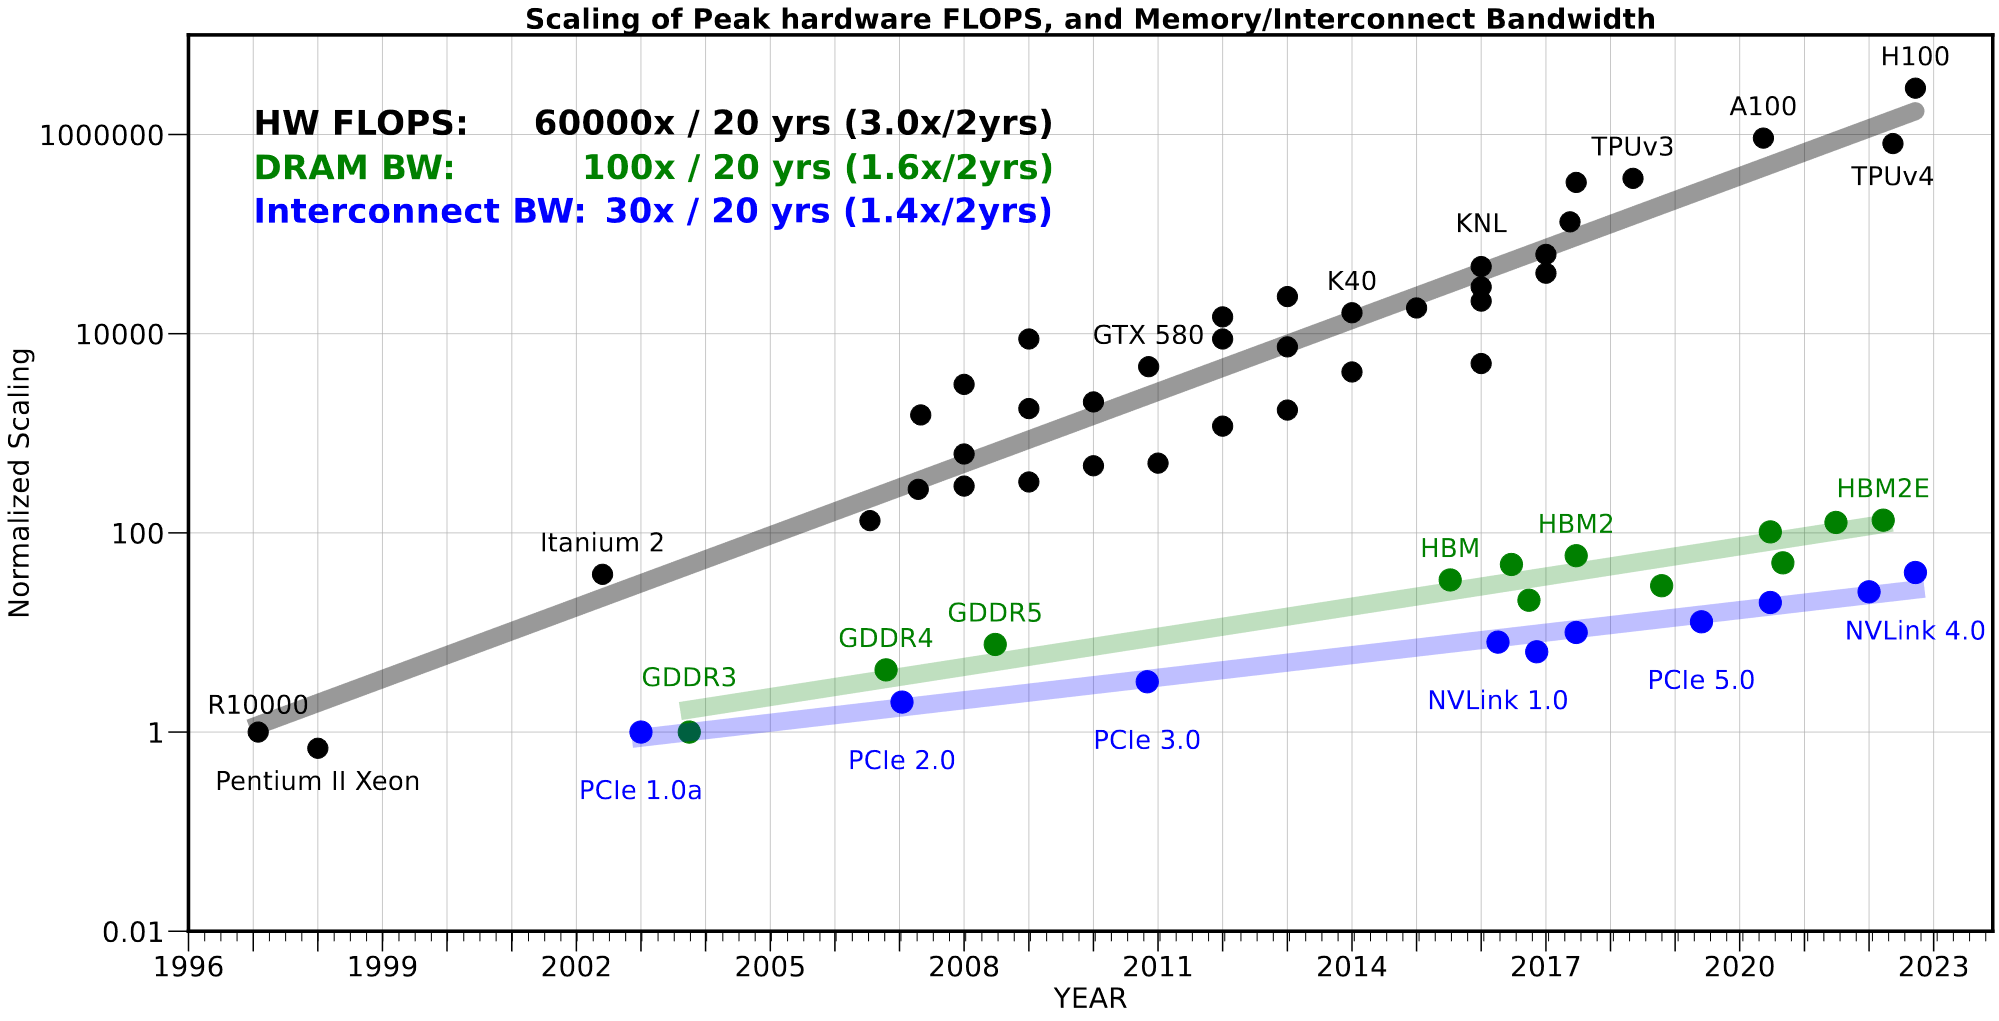
\includegraphics[width=0.8\textwidth]{image.png}
    \caption{Gráfico comparando o avanço do processador versus o avanço da memória em termos de desempenho (performance)}
    \label{fig:memory_wall}
\end{figure}

\subsection*{Resposta:}

\textbf{O processador avança significativamente mais rápido que a memória.} 

Este fenômeno é conhecido como ``Memory Wall'', onde a performance dos processadores cresce cerca de 600 vezes mais rápido que a das memórias DRAM. Este gap representa o principal obstáculo para melhorar a performance dos sistemas computacionais.


\end{document}